\section{Linux Development Tools}
\subsection{Entwicklertools}
\begin{description}
    \item [Integrated Development Environment (IDE) $\rightarrow$ Eclipse] \hfill \\
    Editor, Compiler, Linker, Debugger, etc. \\
    Viele Informationen über Code (-Wall)
    \item [Cross-Plattform und Proprietäre Software (Closed Source)] \hfill \\
    Bsp. Qt (Cross-Plattform)
\end{description}

\subsection{GNU Binutils}
\begin{itemize}
    \item GNU Binary Utils $\rightarrow$ Sammlung von Tools für Software Entwickler (Open Source)
    \item Analyse Objektcode, Bibliotheken, Maschinencode
    \item Erzeugung / Manipulation von Programmen
    \item Um Tools nutzen zu können mit -g (Debugging Flags) kompilieren
\end{itemize}

\subsubsection{c++filt}
\begin{itemize}
    \item Mangled Names anzeigen
    \item CoffeeMachineTest::testBeansFSM() $\rightarrow$ \_ZN17CoffeeMachineTest12testBeansFSMEv
\end{itemize}

\subsubsection{gprof}
\begin{itemize}
    \item Ausführungszeiten von Programmen (Kann in Eclipse integriert werden)
    \item pollt Programm Counter mit 100Hz $\rightarrow$ Grobe Schätzung der Zeit
    \item Besser: valgrind (genauer)
\end{itemize}

\subsubsection{nm}
\begin{itemize}
    \item Zeigt die Symbole (Funktionen / Variablen) im Object File mit Adresse
\end{itemize}
\begin{lstlisting}[style=cpp]
0000000000403d86 T _ZN17CoffeeMachineCtrl13processCoffeeENS_5EventE
\end{lstlisting}

\subsubsection{objdump}
\begin{itemize}
    \item Zeigt Informationen über eine oder mehrere Objektdateien
    \item Z.B. -d $\rightarrow$ Disassembly erstellen
    \item Z.B. -s $\rightarrow$ Disassembly erstellen mit Sourcecode
\end{itemize}
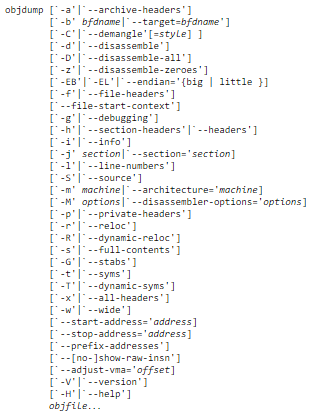
\includegraphics[width=0.5\textwidth]{images/LinuxDevTools/objdump.png}

\subsubsection{size}
\begin{itemize}
    \item Zeigt die Gesamt- und Teilgrössen an
\end{itemize}
\begin{lstlisting}[style=cpp]
$ size CoffeeMachine
text   data  bss   dec    hex   filename
117517 11456 25768 154741 25c75 CoffeeMachine
$
\end{lstlisting}

\subsection{Codeüberdeckung oder -abdeckung (code coverage)}
Bei der Ausführung eines Programms wird versucht, möglichst den ganzen
Code mindestens einmal auszuführen.
\begin{itemize}
    \item Anweisungsüberdeckung (instruction coverage): Jede Anweisung des Programms wird mindestens einmal ausgeführt
    \item Zweigüberdeckung (branch coverage): Jeder Programmzweig wird mindestens einmal durchlaufen
    \item Pfadüberdeckung (path coverage): Jeder Programmpfad, d.h. alle Zweigkombinationen, wird mindestens einmal durchlaufen
\end{itemize}
In der Praxis wird meist nur Anweisungsüberdeckung verlangt,
Zweigüberdeckung wird angestrebt (bei Schleifen explodiert die Anzahl Pfade).\\\\
Überdeckungsgrad \textless 100 \% bedeutet, dass mit den vorhandenen Testfällen nicht alle Anweisungen/Zweige/Pfade ausgeführt werden (ist u.a. auch ein gutes Gütemass für die Testfälle). Folgende Massnahmen können in diesem Fall vollzogen werden: 
\begin{itemize}
    \item Zusätzliche Testfälle definieren
    \item Nicht überdeckter Code analysieren, z.B. mittels Code Inspection
\end{itemize}
Beim nicht ausgeführten Code kann es sich auch um toten Code handeln. Wenn logisch falsch $\rightarrow$ korrigieren bzw. entfernen. Wenn aufgrund defensiven Programmierstil (z.B. default: break) $\rightarrow$ lassen.
\subsubsection{Code Coverage Tool: gcov}
\begin{itemize}
    \item gcov kann in der Kommandozeile oder in Eclipse genutzt werden
    \item gcov zeichnet auf, wie oft eine Codezeile ausgeführt wird
    \item Der Code muss mit den folgenden zusätzlichen Flags compiliert werden:\\-fprofile-arcs -ftest-coverage
    \item Anschliessend kann gcov ein Object- oder Programmfile als Parameter übergeben werden
\end{itemize}
\textbf{Beispiel:}
\begin{lstlisting}[style=bash]
$ gcc -fprofile-arcs -ftest-coverage tmp.c
$ a.out
$ gcov tmp.c
90.00% of 10 source lines executed in file tmp.c
Creating tmp.c.gcov.
$
\end{lstlisting}
Output tmp.c.gcov:
\begin{lstlisting}[style=bash]
-: 0:Source:tmp.c
-: 0:Graph:tmp.gcno
-: 0:Data:tmp.gcda
-: 0:Runs:1
-: 0:Programs:1
-: 1:#include <stdio.h>
-: 2:
-: 3:int main (void)
1: 4:{
1: 5: int i, total;
-: 6:
1: 7: total = 0;
-: 8:
11: 9: for (i = 0; i < 10; i++)
10: 10: total += i;
-: 11:
1: 12: if (total != 45)
#####: 13: printf ("Failure\n");
-: 14: else
1: 15: printf ("Success\n");
1: 16: return 0;
-: 17:}
\end{lstlisting}

\subsection{Performance Profiling - Valgrind}
Valgrind ist eine Tool Suite, die einige Debugging- und Profiling-Tools zur Verfügung stellt.

\subsubsection{Memcheck}
Memcheck detektiert Speichermanagementprobleme
\begin{itemize}
    \item Alle Schreibe- und Lesezugriffe auf den Speicher werden überprüft
    \item malloc/new/free/delete wird überprüft, um Speicherlecks zu detektieren
    \item Arraygrenzen-Überwachung von Memcheck ist für den Heap-Speicher ausgelegt und nicht für Arrays auf dem Stack oder für statische Arrays
\end{itemize}
\subsubsection{Callgrind}
Callgrind kann die Laufzeit eines Programms analysieren
\begin{itemize}
    \item In der Standardkonfiguration wird die Anzahl der ausgeführten Instruktionen aufgezeichnet
    \item Die aufgezeichnete Anzahl der Instruktionen wird zudem mit Sourcecode-Zeilen und Funktionsaufrufen in Beziehung gesetzt
    \item Cachesimulation (Cachegrind) kann aktiviert werden, die weitere Informationen über die Laufzeitperformance des Programms geben kann    
\end{itemize}
\subsubsection{Valgrind-Output}
\begin{itemize}
    \item Das Ergebnis der Laufzeitanalyse wird in eine Datei geschrieben
    \item Die Datei kann dann mit dem Programm KCachegrind visualisiert werden
\end{itemize}


